
\indent \textbf{The Invisible Maze Task.} Participants freely explored an interactive sparse invisible maze environment by walking and probing for virtual visual wall feedback with their hand, delivered by a virtual reality (VR) headset. Four different mazes (Fig. \ref{imt_task} B) were explored in three consecutive runs. Upon collision of the hand with an invisible wall, an illuminated white disc was displayed 30cm behind the collision point parallel to the invisible wall (Fig. \ref{imt_task} C). Due to the complexity of the technical details, please consult~\cite{gehrke2018}. In summary, the task required participants to explore mazes to build a spatial representation of the maze layout.%This behavior is comparable to explorative wall touches in the dark to find your way.

\begin{figure}[h]
\centering
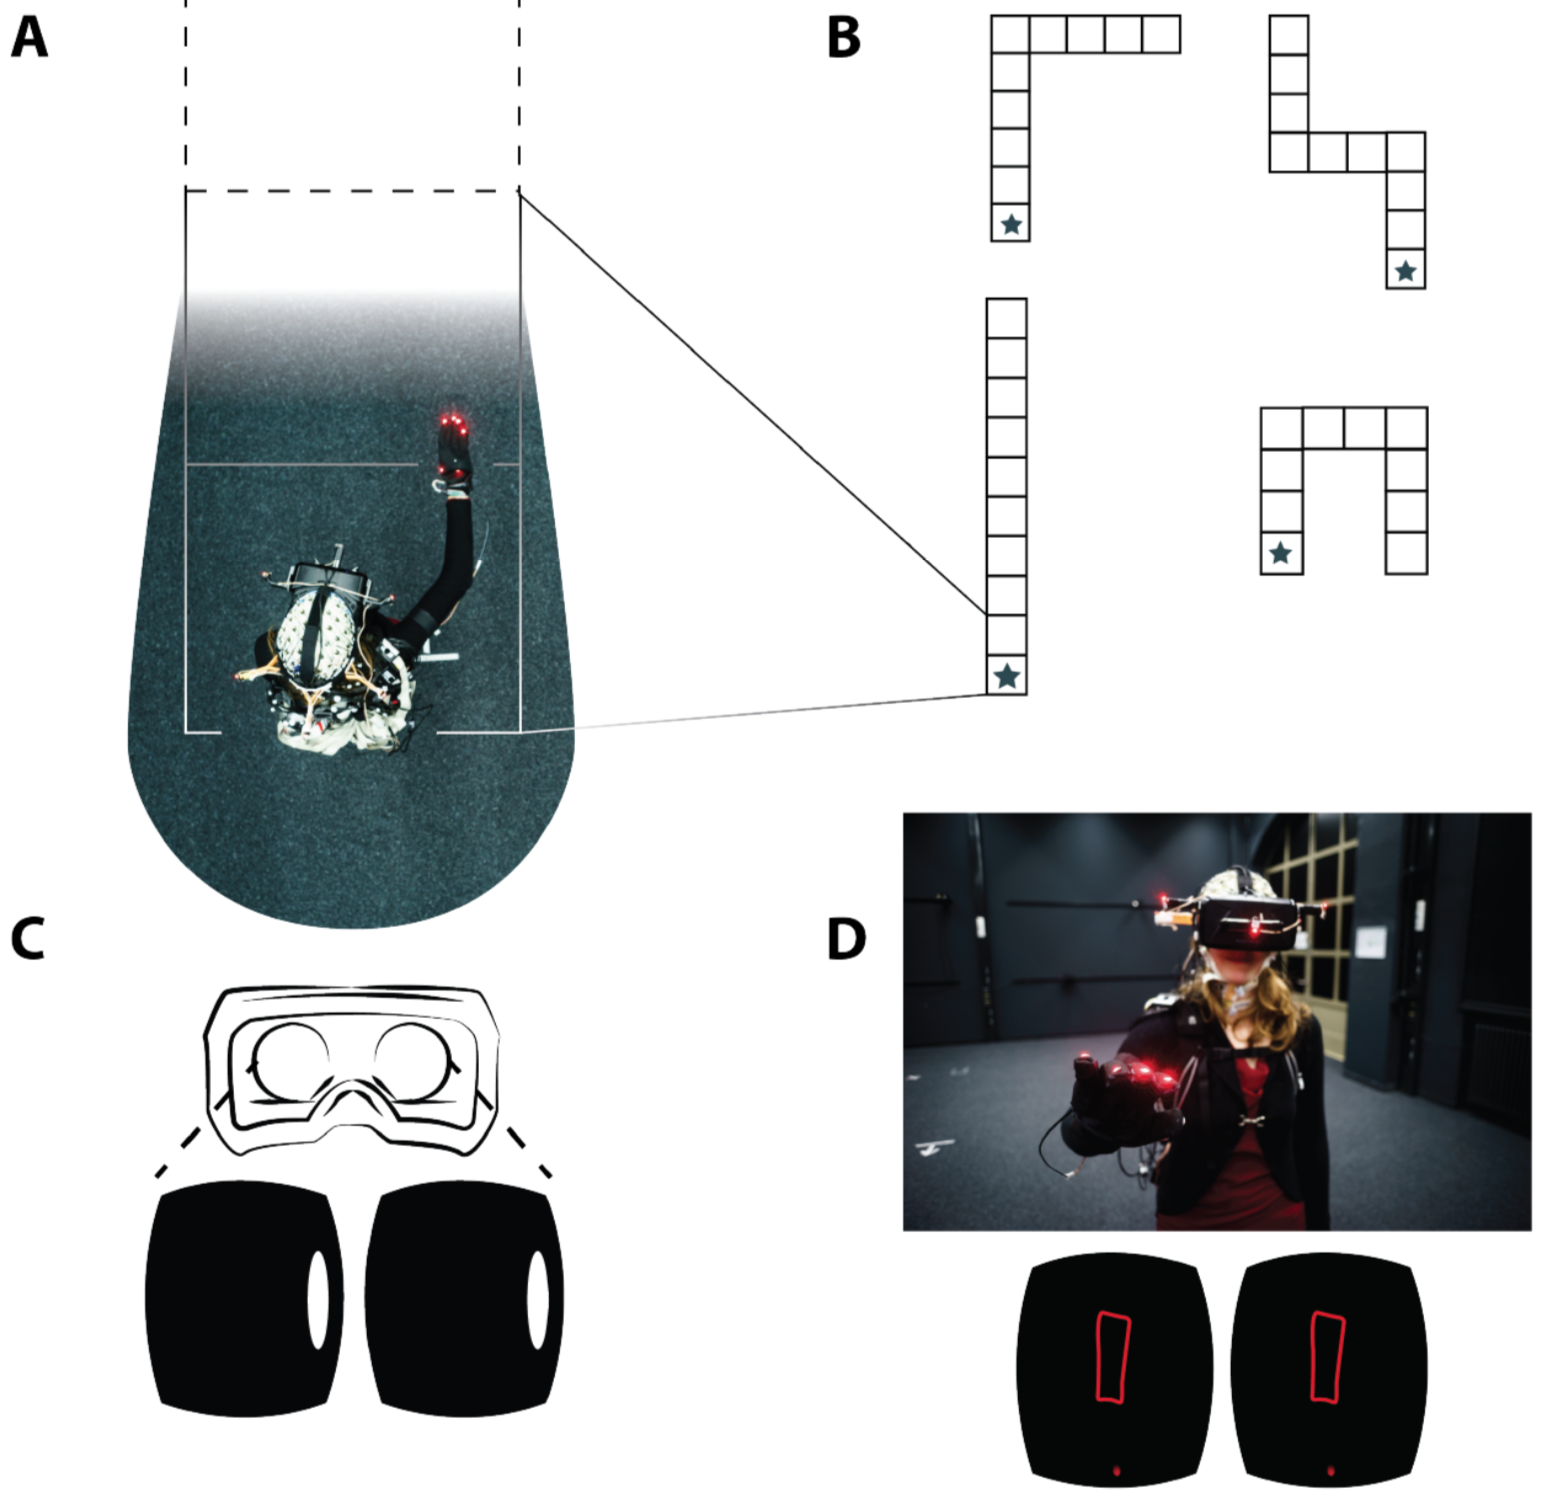
\includegraphics[width=\linewidth]{IMT_Task.png}
\vspace{0pt}
\caption{Invisible Maze Task, \textbf{A} Participant from a bird’s eye view. \textbf{B} Participants are instructed to explore four different mazes and return to the start. \textbf{C} First-person view in binocular ""VR optics"" of a wall touch. \textbf{D} Top: Participants draw a top-down view of the explored maze. Participant is equipped with 160 channels wireless EEG, head-mounted virtual reality goggles and LEDs for motion capture. Bottom: drawn sketch map. Find a detailed description in~\cite{gehrke2018}.}
\label{imt_task}
\end{figure}